\section{Háttérfolyamatok}

\begin{figure}[h!]
  \centering
  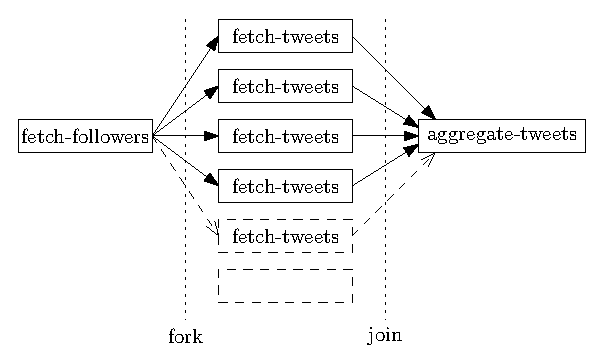
\includegraphics[width=0.75\textwidth]{figures/workflow}
  \caption{Az alkalmazásban lévő háttérfolyamatok összefüggései}
  \label{fig:workflow}
\end{figure}

Az egyes háttérfolyamatok egyszerű Node.JS alkalmazások, amik csatlakoznak
a RabbitMQ szerverhez, és egy adott típusú feladatot végeznek el.

Tetszőleges számú példány elindítható, a kommunikáció hálózaton keresztül
zajlik, így amíg hozzáférnek az üzenetsorhoz, illetve az adatbázishoz,
addig lényegtelen, hogy milyen környezetben futnak.

Alapvetően három fajta feladatot definiáltam, ezek összefüggései
\aref{fig:workflow}. ábrán láthatóak. A feladatok végrehajtásának sorrendje
nem kötött, azonban az egyes folyamatoknam szükségük van egy ponton
szinkronizációra, ennek megoldása nem triviális feladat.

\subsection{Job elosztás}

Az egyes elvégzendő feladatokat a RabbitMQ osztja szét a kliensek között,
akik egymástól teljesen függetlenül képesek működni párhuzamosan,
akár több futtató gépen is.

Az AMQP protokoll támogatja az üzenetek kézbesítésének visszaigazolásos módját,
azaz egy üzenet a célba juttatás esetén csak \emph{unacked} állapoba kerül,
azt a kliensek kell visszaigazolnia. Ezt a kliens az adott feladt elvégzése
után teszi meg, ha a feladatot nem sikerül elvégezni (mert a kliens ezt
explicit kijelenti, vagy a kapcsolat a klienssel megszakad), akkor
az üzenet automatikusan újraütemeződik.

Az AMQP Node.JS binding nem támogatja az üzenetek egyesével történő
elfogyasztását, így az általam használt megoldás egy feliratkozásból,
és egy leiratkozásból áll:

\begin{js}
function* peek(queue) {
  var done;
  var tag;
  queue.subscribe({
    ack: true,
    prefetchCount: 1,
  }, function(message, headers, deliveryInfo, job) {
    queue.unsubscribe(tag).addCallback(function() {
      done(null, {
        message: message,
        headers: headers,
        deliveryInfo: deliveryInfo,
        job: job,
      });
    });
  }).addCallback(function (ok) {
    tag = ok.consumerTag;
  });
  return yield function(cb) {
    done = cb;
  };
}
\end{js}

A feliratkozáskor a kliens egy ún. \emph{consumer tag}-et kap,
ami a feliratkozást azonosítja. Az üzenetek \emph{ack} módban érkeznek,
azaz amíg \verb=prefetchCount= számú üzenet nincs visszaigazolva,
addig a nem kap több üzenetet a kliens.

Ha az első üzenet megérkezett, akkor a kliens az eltárolt consumer tag
alapján elvégzi a leiratkozást, és a hívónak visszaadja a kapott üzenetet,
illetve a hozzá tartozó metaadatokat. Ha a hívó elvégezte a feladatát,
a \verb=job.acknowledge()= metódussal visszaigazolja az üzenetet,
vagy a \verb=job.reject(requeue)=-tel eldobja (és a paraméter értékétől
függően újra beálltja az üzenetsorba).

\subsection{fetch-followers}

A feldolgozás első lépése, hogy a felhasználó követőit lekérdezzük a Twitter
API-ból.

Az API válasz hatására minden egyes követőhöz hozzá kell rendelni
(és beütemezni) egy \emph{fetch-tweets} feladatot,
ami majd az egyes felhasználók tweetjeit fogja megszerezni.

Egy API kérés maximum 1500 követőt képes visszaadni, így ennél nagyobb
mennyiségnél újabb \emph{fetch-followers} feladatot kell beütemezni,
így a \emph{fetch-followers} rekurzívan szerzi meg a felhasználó követőit.

\subsection{fetch-tweets}

A \emph{fetch-tweets} egy adott felhasználó legutolsó tweetjeit kérdezi le,
egy adott időponttól kezdve. A tervezés során úgy határoztam, hogy az egyes
felhasználóknak csak az utolsó két hétben publikált tweetjeit kérdezem le,
vagy amennyit a rendszer megenged (3200 tweet, szerencsére ez minden
esetben elegendőnek bizonyult).
Kezdetben a legutolsó 200 tweetet kérdezi le a rendszer,
majd ha ezek közül egyik tweet sem régebbi 2 hétnél,
akkor a készít egy új \emph{fetch-tweets} jobot, ami a legrégebbi
(de még mindig két hétnél frissebb) tweet előtti üzeneteket tölti le.
Így előbb-utóbb rekurzív módon minden szükséges tweet letöltésre kerül.

\subsection{aggregate-tweets}

Ha az adatok begyűjtése megtörtént, akkor a rendszer elvégzi az összegyűjtött
tweetek aggregálását. A folyamat egyrészt detektálja, hogy valóban el kell-e
végezni az aggregálást (azaz a felhasználónál nem maradt már \emph{pending}
állapotú feladat): ha még további adatok letöltése szükséges,
akkor befejezi a futást.
Amint az utolsó job is lefutott, megtörténik a tényleges aggregálás.
Ehhez le kell kérdezni az adatbázisból az összegyűjtött tweeteket, majd
azokat csoportosítani a létrehozásuk ideje alapján, végül az ezekbe a
csoportokba eső üzeneteket kell megszámolni. Az eredményt el kell tárolni,
hogy azt a frontend alkalmazás a felhasználónak később meg tudja mutatni.
